\chapter{Tree Refinement}
\label{chap:tree}
% 0.5 Seiten

	With the existing capabilities of \ac{GCG} presented in the previous chapter, we continue with the main contributions of this thesis:
	
	\begin{itemize}
		\item A new module which is integrated into the detection framework of \ac{GCG} for reverse engineering semantic groupings of the original formulation.
		\item Additional auxiliary classifiers which implement constraint and variable classification based on information not currently used including examples of \textit{when} they are crucial detecting semantics.
	\end{itemize}

	This chapter is divided into three main section:
	
	\begin{enumerate}
		\item A short summary about the available information we have access to.
		\item What the motivation and goals are why and how we aim to process this information.
		\item The concrete algorithm and its most integral parts.
	\end{enumerate}
	
	Some concrete details about the implementation itself are not subject of the following sections, but are discussed in Chapter \ref{chap:impl}.

	\clearpage

	\section{Information}
	% 1 Seite
	
	\begin{figure}[ht!]
		\centering
		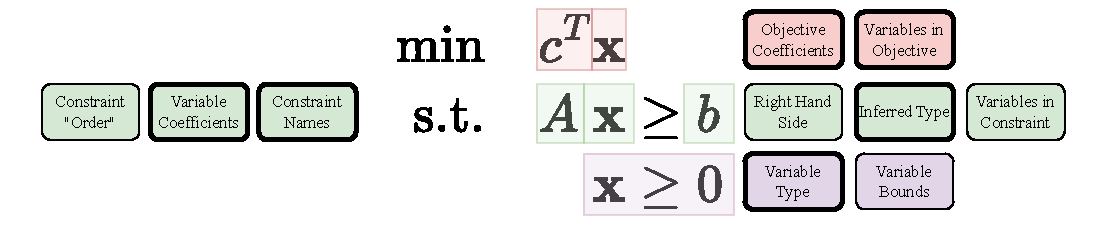
\includegraphics[scale=0.8]{Bilder/DrawIO/model_information}
		\caption{All parts of a model that contain useful information for semantic grouping of constraints and variables. Elements with a thick border are already used as a key concept in one of the existing detectors.}
		\label{fig:tree:information}
	\end{figure}
	
	Before we present any algorithmic details, we give an overview about the available information.
	
	\begin{enumerate}
		\item \textbf{Objective}: For the objective functions, information about the participating variables and their coefficients is available. For some models e.g. for Bin-Packing, this information alone is sufficient to partition the variables.
		\item \textbf{Coefficients}:
		The use of coefficients to classify constraints and variables was already in discussed in Section \ref{chap:gcg:classifiers}.
		\item \textbf{Bounds}: For all variables $lb \leq x \leq ub$ information about their lower- and upper-bounds is available.
		Furthermore, the left- and right-hand-side of linear constraints $lhs \leq \sum_i a_i x_i \leq rhs$ are available as well.
		\item \textbf{Types}: Variable types such as \textit{Integer} are usually stated explicitly in the input format. If not, then information about the variable bounds can be used to deduce a type, e.g. $0 \leq x \leq 1$ is a strong indicator that $x$ is a \textit{Binary} variable.
		\item \textbf{Names}: If specified by the modeler, then variables and constraints might have meaningful names which can be used as a strong indicator which constraints and variables belong to the same group.
		\item \textbf{Order}: In contrast to other kinds of information, the constraint \enquote{order} is no intrinsic property of the model itself. With the term \enquote{order}, we refer to the order of the constraints as specified in the input format. When a model is created e.g. via. a script, constraints are usually added in \textit{blocks} by the modeler. This information is used in Section \ref{chap:tree:classifiers:voting} to conceptualize a classifier based on that.
	\end{enumerate}
	
	\section{Motivation}
	% 2 Seiten
	
		\clearpage
	
	\section{Classifiers}
	% 2 Seite
	
		In the following Sections we describe different classifiers which are not yet implemented in \ac{GCG} but could potentially provide new information about the model.
		
		\subsection{Bounds}
			
			When considering bounds, we differentiate between two types:
			\begin{enumerate}
				\item Bounds of a single variable $\text{lower bound} \leq x \leq \text{upper bound}$
				\item Constraint Bounds, $\text{lhs} \leq \sum a \mathbf{x} \leq \text{rhs}$
			\end{enumerate}
			
			\subsubsection{Variable bounds}
			
				
				
			\subsubsection{Constraint bounds}
			
			\clearpage
		
		\subsection{Relaxed MIPLIB types}
			
				\begin{table}[ht!]
				\centering
				\begin{tabular}{l|l|l|l}
					\textbf{Nr.} & \textbf{Type} & \textbf{Linear Constraint} & \textbf{Notes} \\
					\hline
					\hline
					1 & Empty & $\emptyset$ & - \\
					2 & Free & $-\infty \leq x \leq \infty$ & No finite side. \\
					3 & Singleton & $a \leq x \leq b$ & - \\
					4 & Aggregation & $ax + by = c$ & - \\
					5 & Precedence & $ax - ay \leq b$ & $x$, $y$ have same type. \\
					6 & Variable Bound & $ax + by \leq c$ & $x \in \{0, 1\}$ \\
					7 & Set Partitioning & $\sum 1 x_i = 1$ & $\forall i: x_i \in \{0, 1\}$ \\
					8 & Set Packing & $\sum 1 x_i \leq 1$ & $\forall i: x_i \in \{0, 1\}$ \\
					9 & Set Covering & $\sum 1 x_i \geq 1$ & $\forall i: x_i \in \{0, 1\}$ \\
					10 & Cardinality & $\sum 1 x_i = b$ & $\forall i: x_i \in \{0, 1\}, b \in \mathbb{N}_{\geq 2}$ \\
					11 & Invariant Knapsack & $\sum 1 x_i \leq b$ & $\forall i: x_i \in \{0, 1\}, b \in \mathbb{N}_{\geq 2}$ \\
					12 & Equation Knapsack & $\sum a_i x_i = 1$ & $\forall i: x_i \in \{0, 1\}, b \in \mathbb{N}_{\geq 2}$ \\
					13 & Bin Packing & $\sum a_i x_i + ay \leq a$ & $\forall i: x_i, y \in \{0, 1\}, b \in \mathbb{N}_{\geq 2}$ \\
					14 & Knapsack & $\sum a_i x_i \leq b$ & $\forall i: x_i \in \{0, 1\}, b \in \mathbb{N}_{\geq 2}$ \\
					15 & Integer Knapsack & $\sum a_i x_i \leq b$ & $\forall i: x_i \in \mathbb{Z}, b \in \mathbb{N}$ \\
					16 & Mixed Binary & $\sum a_i x_i + \sum p_j s_j \; \{\leq, =\} \; b$ & $\forall i: x_i \in \{0, 1\}, \forall j: s_j \; \mathrm{continuous}$ \\
					17 & General Linear & $\sum a_i x_i \; \{\leq, \geq, =\} \; b$ & No special structure.
				\end{tabular}
				\caption{The structure of all 17 constraint types MIPLIB keeps track of.}
				\label{table:constypes:relaxedd}
			\end{table}
			
			This table
			
			\clearpage
			
		\subsection{Ordered Voting}
		\label{chap:tree:classifiers:voting}
		
			Ordered Voting
		
			\clearpage
			
		\subsubsection{Co-occurence clustering}
		\label{chap:tree:classifiers:cooccurence}
		
			Co
			
			\clearpage
		
%	\section{Tree Refinement}
%	% 4 Seiten
%	
%		\begin{figure}[ht!]
%			\centering
%			\includesvg{Bilder/Hierarchy/hierarchy_binpack_NOP}
%			\caption{Test}
%			\label{fig:tree:binpackNOP}
%		\end{figure}
		
	\section{Strategies}
	
		Strategies are \textit{the} central building block of the algorithm and are responsible for refining sets of constraints or variables.
		Let $U$ be a the total set of constraints or variables.
		Each strategy gets a single set $S \subseteq U$ as input and produces a partition $\pi_S \in \Pi(S)$ of that set as output.
		Each set $A_i \in \pi_S$ corresponds to one child node.
		Conceptually, each strategy can be seen as a materialization of a specific splitter function as defined in Section \ref{chap:prelims:partitionref}.
		In the following, we differentiate between re-callable and non re-callable strategies. The former type may be called more than once in any given sub-tree, as the result may depend on the set that is being refined.
		
		\clearpage
	
		\subsection{Slice (Partition)}
		
			\begin{figure}[ht!]
				\centering
				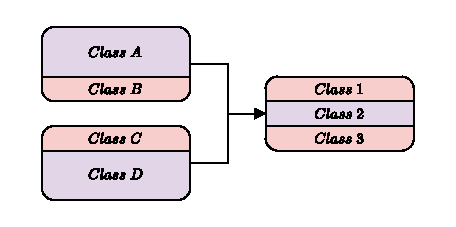
\includegraphics[scale=1.2]{Bilder/DrawIO/strat_slicing_pdf}
				\caption{A simplified illustration assuming that constraint in both partitions can be rearranged into continuous blocks, thus \enquote{slicing} the partitions into different-sized chunks. The output partition inherits all these slices.}
				\label{fig:tree:strat:slice}
			\end{figure}
		
			Slicing strategies are the most simple type of strategy.
			Given two partition $\pi, \pi' \in \Pi(U)$, we define the \textit{combined partition} $\pi \sqcap \pi'$ as follows:
			%
			\begin{equation}
				\label{eq:tree:strat:slice:overlay}
				\pi \sqcap \pi' = \{ A_i \cap B_j \mid A_i \in \pi, B_j \in \pi' \} \setminus \emptyset
			\end{equation}
			%
			This concept is illustrated in Figure \ref{fig:tree:strat:slice}.
			Because strategies only refine single sets and not whole partitions, Equation \ref{eq:tree:strat:slice:overlay} always degenerates to $\pi_{slice} \sqcap \{ S, U \setminus S \}$ for some partition $\pi_{slice} \in \Pi(U)$ and a set $S$ we want to refine.
			The result is then restricted to elements of $S$, which yields a partition of $S$.
			More formally, this strategy can be expressed as Function \ref{eq:tree:strat:slice:function} and computed efficiently using Algorithm \ref{algo:tree:strat:slice}. 
			\begin{equation}
			\label{eq:tree:strat:slice:function}
				f(\pi_{splitter}, S) = \left\{ A_i \cap S \mid A_i \in \pi_{splitter} \right\}
			\end{equation}
		
			\begin{algorithm}[ht!]
				\centering
				\begin{algorithmic}
					\Require Partition $\pi = \{ A_1, A_2, \ldots, A_k \}$, set $S \subseteq U$, function $f_C: U \mapsto \mathbb{N}$ for $C = \{ C_1, C_2, \ldots \} \in \Pi(U)$ mapping $u \in U$ to $C_i$ iff $u \in C_i$
					\Ensure Partition of $S$ according to Function \ref{eq:tree:strat:slice:function}.
					\Statex
					%
					\Function{strategySlice}{$\pi, S$}
						\State $\pi_{out} \gets$ list of $k$ empty sets $B_1, B_2, \ldots, B_k$
						\For{$s \in S$}
							\State $i \gets f_S(s)$
							\State $B_i \gets B_i \cup \{ s \}$
						\EndFor
						\State Remove empty sets from $\pi_{out}$
						\State \Return $\pi_{out}$
					\EndFunction
				\end{algorithmic}
				\caption{If a lookup table represented by function $f$ is available, then Function \ref{eq:tree:strat:slice:function} can be implemented in O($|S|$).}
				\label{algo:tree:strat:slice}
			\end{algorithm}
			
			\clearpage
		
		\subsection{Slice (Covering)}
		
			This strategy is functionally equivalent to the refinement method \enquote{fast} from \cite{salvagninDetectingSemanticGroups2016}.
			The name most likely stems from an algorithm informally described a fast algorithm based on bucket sort to implement such a partition refinement algorithm.
			
			\clearpage
		
		\subsection{Recursive}

			The \textit{recursive} strategy is the the only strategy which utilizes the full blown partition refinement framework.
			
			\clearpage
			
	
	\section{Scoring}
	% 1 Seite
	
		\subsection{Constraint Names}
		
			\begin{algorithm}[ht!]
				\centering
				\begin{algorithmic}
					\Require Name of a constraint
					\Ensure Relevant semantics of the constraint name if the name adheres 
					\Statex
					%
					\Function{extractSemanticPart}{$name$}
						\State ${name}_{new} \gets name$
						\State ${name}_{old} \gets name$
						\Repeat
							\State ${name}_{old} \gets name$
							\State $start \gets$ Position of opening character e.g. $\lbrack$, \{, (, $\ldots$
							\State $end \gets$ Position of corresponding closing character e.g. $\rbrack$, \}, ), $\ldots$
						\Until{${name}_{new} = {name}_{old}$}
					\EndFunction
				\end{algorithmic}
				\caption{}
				\label{algo:tree:scoring:nameheur}
			\end{algorithm}
			\todo{WIP}
			
			\clearpage
			

		\subsection{Ground Truth based}
		% 1 Seite
		
			Ground-Truth
		
			\clearpage
	
		\subsection{Connected Block Score}
		% 1 Seite
	
			Connected

			\clearpage